% =============================================================================
%  Part VIII -- Predictions and falsification
% =============================================================================

This part sets out what Causal Physics predicts, how each prediction is to be tested, and what would
falsify the theory. It is the programme for the next round of tests: every entry below is formulated so
that a test with a criterion fixed in advance can be written for it.

% =============================================================================
\section{What counts as a prediction}\label{sec:what-prediction}
% =============================================================================

A result is a \emph{prediction} only if it is fixed before the comparison and nothing in it was
calibrated on the data it is compared with. The results of the theory fall into three classes:
\begin{enumerate}
\item \textbf{Consistency with general relativity.} In the regime where geometry describes the order, the
  theory reproduces general relativity at the linear order and adopts it beyond. Agreement with the
  classical tests is required, not predicted.
\item \textbf{Predictions of the discreteness.} Deviations from general relativity whose \emph{shape} is
  fixed by the Benincasa--Dowker kernel and whose \emph{scale} is the single free parameter $\ell_k$.
  These are the predictions of the theory. Data either bound $\ell_k$ or detect the deviation.
\item \textbf{Structural statements.} Properties of the substrate that hold independently of $\ell_k$:
  Lorentz invariance, sharp images of distant sources, the area law of horizons.
\end{enumerate}

% =============================================================================
\section{Consistency with general relativity}\label{sec:consistency}
% =============================================================================

\begin{center}
\begin{tabularx}{\linewidth}{>{\raggedright\arraybackslash}p{3.6cm}>{\raggedright\arraybackslash}X>{\raggedright\arraybackslash}p{4.6cm}}
\toprule
quantity & origin in Causal Physics & status\\
\midrule
$\gamma=1$ & throughput principle; tensor coupling in 3+1; action of the order & derived; F7.1c raw $1.000\pm0.045$; $\cA$, $\cB$, $\cC$ emerge, $\gamma(0)=0.997$--$1.000$ (F6.8a, F6.8b2, F6.8c2)\\
$\beta=1$ & general-relativistic completion; logarithmic static section & follows from the completion; the logarithm is chosen to match it\\
frame dragging & response in the rest frame of each flow & derived; F7.4a\\
pressure gravitates as $\rho+3p$ & coupling to $T_{ab}$ & derived; F7.4a\\
quadrupole radiation, two polarisations & tensor field, GR completion & derived\\
equivalence principle & motion along the longest histories & derived; free fall along longest chains F5.1d (2+1)\\
Lorentz invariance & sprinkled substrate & structural\\
\bottomrule
\end{tabularx}
\end{center}

% =============================================================================
\section{The window of the non-locality scale}\label{sec:window}
% =============================================================================

Every prediction of the discreteness is a function of $\ell_k$, and $\ell_k$ is not free in the whole range
from the Planck length to laboratory scales.

\paragraph{Existing bounds.} The non-locality of causal set d'Alembertians has been confronted with data
for fields that propagate with the non-local operator. Comparing non-local relativistic effective field
theories with collider data at $8$\,TeV gives $\ell_k\lesssim10^{-19}$\,m, and the ground state of an
opto-mechanical oscillator gives an independent $\ell_k<2\times10^{-15}$\,m~\cite{Belenchia2016opto}.
In Causal Physics matter is a flow that carries its four-velocity, not a field propagated by $B_\epsilon$,
so whether these bounds apply to the scale of the gravitational sector depends on the matter sector,
which is open. If the same $\ell_k$ governs both, $\ell_k\lesssim10^{-19}$\,m. \stat{open}

\paragraph{Consequence for the local corrections.} For $\ell_k\lesssim10^{-19}$\,m the local correction of
Sec.~\ref{sec:bdaction}, of relative size $(k\ell_k)^2\ln(1/k\ell_k)$, is below $10^{-28}$ at the shortest
distance at which gravity is measured, $52\,\mu$m~\cite{Lee2020}: unobservable.

\paragraph{Consequence for the age term.} The age term is not suppressed in the same way. Its relative size
$\delta\simeq c_T\,k^3\ell_k^2\,T$ grows with the age $T$, and with $k=1/L$ it becomes of order one at the length
\begin{equation}\label{eq:Lstar}
  L_*=\big(c_T\,\ell_k^2\,T\big)^{1/3},\qquad c_T=0.1035 .
\end{equation}
Requiring $\delta<10^{-2}$ at $L$ gives $\ell_k\lesssim\sqrt{\delta L^3/(c_T T)}$. The outcome depends on what
$T$ is:
\begin{center}
\small
\begin{tabular}{lcccc}
\toprule
reading of $T$ & $T$ (m) & bound on $\ell_k$ & $L_*$ & $L_*$\\
 & & from $L=52\,\mu$m & ($\ell_k=\ell_P$) & ($\ell_k=10^{-19}$\,m)\\
\midrule
age of the universe & $1.3\times10^{26}$ & $1\times10^{-20}$\,m & $1.5\times10^{-15}$\,m & $51\,\mu$m\\
age of Earth's field & $4.3\times10^{25}$ & $2\times10^{-20}$\,m & $1.0\times10^{-15}$\,m & $35\,\mu$m\\
one year & $9.5\times10^{15}$ & $1\times10^{-15}$\,m & $6\times10^{-19}$\,m & $21$\,nm\\
one day & $2.6\times10^{13}$ & $2\times10^{-14}$\,m & $9\times10^{-20}$\,m & $3$\,nm\\
\bottomrule
\end{tabular}
\end{center}
If $T$ is cosmological, short-range tests of gravity probe $\ell_k$ at the level of collider bounds, and the
theory says where the deviation sits: at $L_*$, which for $\ell_k=10^{-19}$\,m lies at tens of micrometres,
the range of current torsion balances. If $T$ is the age of a laboratory source, the age term is out of reach.
What $T$ is (Sec.~\ref{sec:discreteness-predictions}, P2) therefore decides whether the theory is testable
at short distances now (Fig.~\ref{fig:window}). \stat{derived; conditional on the reading of $T$}

\begin{figure}[t]
  \centering
  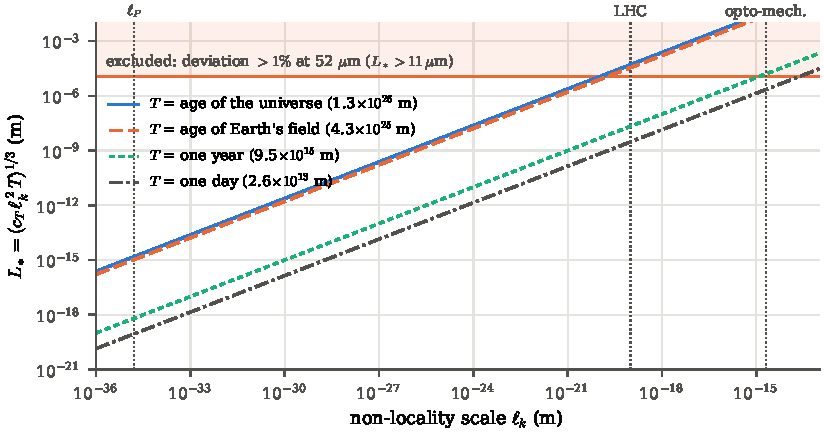
\includegraphics[width=\textwidth]{figures/fig_window.pdf}
  \caption{The window of the non-locality scale, Eq.~\eqref{eq:Lstar}: the length $L_*$ at which the age term becomes of
order one, against $\ell_k$, for the four readings of $T$. Shaded: excluded by short-range tests of gravity if
the deviation must stay below $1\%$ at $52\,\mu$m ($L_*>11\,\mu$m). Dotted: the Planck length and the bounds on
$\ell_k$ from colliders and opto-mechanics (if the same $\ell_k$ governs matter). The curves use the linear age
term of the conformal sector, $c_T=0.1035$ (caveat (i)).}\label{fig:window}
\end{figure}

\paragraph{Caveats.} (i) The estimate uses the linear age term of the conformal sector. The optical sector
weakens faster than linearly within the computed range ($kT\le24$, Sec.~\ref{sec:optical}); if this persists
as $kT\to\infty$, the breakdown moves to larger scales and the bounds become stronger. The asymptotic form decides the far-field law. (ii) In the mixed sector the age term is $1.78$ times stronger than in the
conformal one (Sec.~\ref{sec:mixed}); a covariant action cannot do this, and the difference may come from
the age cut rather than from the action. (iii) At $L_*$ the expansion in the age term breaks down, and what
happens there (Sec.~\ref{sec:discreteness-predictions}, P3) is open. The numbers above are orders of
magnitude, not a verdict.

% =============================================================================
\section{Predictions of the discreteness}\label{sec:discreteness-predictions}
% =============================================================================

\subsection{P1: the static field of a point mass near \texorpdfstring{$\ell_k$}{l\_k}}

The static field of a point mass is fixed by the three coefficients $\cA$, $\cB$, $\cC$ of the static
quadratic form of the action of the order (Sec.~\ref{sec:mixed}), without assuming covariance:
\begin{equation}
  \gamma(k,T)=\frac{\cB}{2\cC}-1,\qquad
  \frac{\Phi(k)}{\Phi_{\rm GR}(k)}=\frac{-2}{\cA-\cB^2/(4\cC)} .
\end{equation}
\begin{itemize}
\item \emph{Known:} the conformal coefficient $\cA=6\hat K(k,T)$, with
  $K_{\rm loc}=1-(k\ell_k)^2[4.0\ln(1/k\ell_k)+0.9]+\dots$ for $k\ell_k\le0.1$ and the values of
  Sec.~\ref{sec:bdaction} beyond; the mixed coefficient $\cB=8\hat K_{ab}(k,T)$, equal to $8\hat K$ at leading
  order and larger by $\simeq8\times0.46\,(k\ell_k)^2$ beyond it (Sec.~\ref{sec:mixed}); the optical coefficient
  $\cC=2\hat K_{bb}(k,T)$, with $\cC(k\to0)=2.002$ and an age dependence that grows faster than linearly in the
  computed range (Sec.~\ref{sec:optical}).
\item \emph{To compute:} the asymptotic form of the optical age term, $kT\to\infty$.
\item \emph{Prediction:} the potential $\Phi(r)$ and $\gamma(r)$ of a point mass as functions of
  $r/\ell_k$, by Fourier inversion. The shape is fixed; only $\ell_k$ is free.
\item \emph{Test:} laboratory searches for deviations from the inverse-square law at sub-millimetre
  distances (torsion balances~\cite{Lee2020}), and light deflection and Shapiro delay at the largest $k$
  accessible. If $\ell_k$ obeys the existing bounds (Sec.~\ref{sec:window}), the local part of P1 is out of
  reach and its observable content is the age term.
\item \emph{Falsification:} if the predicted shape is excluded by the data for every $\ell_k$ above the
  discreteness length $\ell$, the theory fails.
\end{itemize}

\subsection{P2: the age term}

A static field that has existed for a time $T$ responds more weakly at wavenumber $k$ by the relative
amount
\begin{equation}
  \frac{\delta\hat K}{\hat K}\simeq-0.10\,k^3\ell_k^2\,T\qquad(c=1).
\end{equation}
\begin{itemize}
\item \emph{Status:} derived analytically and confirmed by the full computation to $2\%$, in the static
  conformal sector (F6.8a). In the mixed sector it is $1.78$ times larger, $c_{T,ab}\simeq0.195$
  (F6.8b2): the age term does not enter the sectors in covariant proportion. In the optical sector it grows
  faster than linearly within the computed range, $kT\le24$ (F6.8c2), with a form the data do not fix; it
  therefore shifts $\gamma$ as well as the strength of the field. Its form as $kT\to\infty$ is open.
\item \emph{Open:} what $T$ is physically (age of the field, of the source, or the cosmological past),
  and the form of the term in the full static propagator.
\item \emph{Consequence:} requiring a relative deviation below $\delta$ at scale $L$ gives
  \begin{equation}
    \ell_k\lesssim\sqrt{10\,\delta\,L^3/T},
  \end{equation}
  e.g.\ $\ell_k\lesssim1$\,mm from the field of the Earth at the scale of its radius ($\delta=10^{-2}$). At the
  shortest tested distance, $52\,\mu$m, the bound ranges from $10^{-20}$\,m (cosmological $T$) to
  $2\times10^{-14}$\,m ($T$ of one day); Sec.~\ref{sec:window}.
\item \emph{Caveat:} the age term enters the conformal and mixed sectors in a non-covariant proportion; it may
  come from the way the past is cut at age $T$ rather than from the action. A test of this is planned
  (F6.8d).
\item \emph{Test:} comparison of the strength of gravity of fields of different ages at the same scale,
  e.g.\ freshly assembled laboratory masses against the field of the Earth.
\end{itemize}

\subsection{P3: the static pole of the spin-0 channel}

The spin-0 propagator has a static pole where $\hat K=0$. Without the age term it lies at a wavelength
of $12.7\,\ell_k$; with it, at the length scale $L_*=(0.1\,\ell_k^2T)^{1/3}$ of Eq.~\eqref{eq:Lstar}, which for
$T$ equal to the age of the universe is $\sim10^{-15}$\,m for a Planckian $\ell_k$ and $\sim50\,\mu$m for
$\ell_k=10^{-19}$\,m. Whether the pole signals a standing wave, an
instability of the static sector, or the limit of validity of the expansion is open. \stat{open}

\subsection{P4: the cosmological constant}

The fluctuation of the number of events gives a cosmological constant of the observed order of magnitude
that varies over cosmic time~\cite{Ahmed2004}. This is a known prediction of causal set theory that
Causal Physics shares. \stat{open}

% =============================================================================
\section{Structural predictions}\label{sec:structural}
% =============================================================================

\begin{itemize}
\item \textbf{Exact Lorentz invariance of the substrate.} No preferred frame at any scale. A detected
  violation of Lorentz invariance would contradict Axiom~\ref{ax:substrate}. A Lorentz-invariant discrete
  substrate can still make particles diffuse slowly in momentum (``swerves''~\cite{DowkerHensonSorkin2004});
  for flows that carry their four-velocity this has not been computed. \stat{open}
\item \textbf{No blurring of distant point sources by the discreteness.} Influence on the light cone
  passes no intermediate events, so the images of distant quasars and gamma-ray bursts are not blurred
  by the substrate. Observed sharp images agree with this; a detected discreteness-induced blurring would
  contradict it.
\item \textbf{Horizon entropy proportional to proper area,} with the discreteness length tied to $G$
  through $s_0$ (Sec.~\ref{sec:bridge}).
\end{itemize}

% =============================================================================
\section{Falsification}\label{sec:falsification}
% =============================================================================

The theory is falsified, in the sense that its present form must be abandoned, if any of the following
holds:
\begin{enumerate}
\item a deviation from general relativity is measured in the classical tests (light deflection,
  Shapiro delay, perihelion advance, frame dragging, binary pulsars, gravitational-wave polarisations)
  at scales far above any admissible $\ell_k$;
\item the $\nu^2$ sector of the discrete action gives a long-wavelength coefficient $\cC$ different from
  $2$: then $\gamma=\cB/(2\cC)-1\neq1$ at large scales, $\gamma=1$ does not follow from the action of the order,
  and the substrate rule is an independent postulate (checked: $\cB\to7.983$, $\cC\to2.002$, passed);
\item the static field of a point mass predicted from the three coefficients $\cA$, $\cB$, $\cC$ is excluded by
  short-range gravity data for every $\ell_k\ge\ell$;
\item a violation of Lorentz invariance of the substrate is detected;
\item the images of distant point sources are found blurred in a way attributable to the discreteness
  of spacetime.
\end{enumerate}

% =============================================================================
\section{The next tests}\label{sec:next-tests}
% =============================================================================

\begin{center}
\begin{tabularx}{\linewidth}{>{\raggedright\arraybackslash}p{1.3cm}>{\raggedright\arraybackslash}X>{\raggedright\arraybackslash}p{3.0cm}}
\toprule
test & question & needs\\
\midrule
F6.8e & the asymptotic age term of the optical sector, $kT\to\infty$ (analytic, as for $c_T$) & F6.8c2\\
F6.8d & the differences between the sectors beyond leading order: from the age cut or from the action? & F6.8b2\\
F8.1 & $\Phi(r)$, $\gamma(r)$ of a point mass in units of $\ell_k$; comparison with short-range data & F6.8e\\
F8.8 & the physical meaning of the age $T$; fields of different ages & theory of $T$\\
F6.9 & the age term in the full static propagator & F6.8c\\
\bottomrule
\end{tabularx}
\end{center}
Each of these will be registered with its criterion before it is run, and its outcome reported whatever it
is.
